\documentclass[11pt]{article}


\usepackage{preamble}

\title{Error Correcting Codes, Hardness Amplification and Boosting.}
\date{}

\begin{document}
    
\noindent Error Correcting Codes, Hardness Amplification and Boosting \hfill  CS 250, Winter 2025\\
\hrule


\section{Introduction}

\tableofcontents


\section{Preliminaries}

\section{Hardness Amplification with ECCs}

\begin{definition}{3.x}
    We say that a function $G : \pmo^\ell \rightarrow \pmo^{n}$ is an $(\ell, n)$-PRG if, for any size $n$ circuit $C$ over $n$ inputs, 
    \begin{equation*}
        \left|\Pr_{x \backsim U_n}[C(x)] - \Pr_{x \backsim U_s}[C(G(s))]\right| < \frac{1}{10}.
    \end{equation*}
\end{definition}

The parameter $\ell$ is the seed length.

\begin{assumption}{1} \label{a-1}
    There exists a function $f : \pmon \rightarrow \pmo$ such that $f$ can be computed in time $2^{O(n)}$, but there exists some $\delta > 0$ such that 
    \begin{equation*}
        \Corr\left(f, 2^{\delta n}\right) < 1.
    \end{equation*}
\end{assumption}

\begin{assumption}{2} \label{a-2}
    There exists a function $f : \pmon \rightarrow \pmo$ such that $f$ can be computed in time $2^{O(n)}$, but there exists some $\delta > 0$ such that 
    \begin{equation*}
        \Corr\left(f, 2^{\delta n}\right) < .9.
    \end{equation*}
\end{assumption}

\begin{assumption}{3} \label{a-3}
    There exists a function $f : \pmon \rightarrow \pmo$ such that $f$ can be computed in time $2^{O(n)}$, but there exists some $\delta > 0$ such that 
    \begin{equation*}
        \Corr\left(f, 2^{\delta n}\right) < 2^{-\Omega(n)}.
    \end{equation*}
\end{assumption}

We will prove that, given a worst case hard function $f$, we can transform it into an average case $f'$.

\begin{theorem}{3.x} If there exists a function $f$ satisfying the worst case hardness assumption, there exists a function $f'$ satisfying the average case hardness assumption.

\end{theorem}

\subsection{Why Hardness Amplification?}

\begin{theorem}{3.x} Suppose that $G$ is a $(O(\log n), n)$-PRG computable in $\poly(n)$ time. Then $\P = \BPP$.
\end{theorem}

\subsubsection{A Simple PRG}

\begin{theorem}{3.x}
    Given the average case hardness assumption, there exists a $(n - 1, n)$-PRG.
\end{theorem}

\subsubsection{The Nisan-Wigderson Generator}

\begin{theorem}{3.x}
    Given the average case hardness assumption, there exists a $(O(\log n), n)$-PRG.
\end{theorem}

\begin{center}
    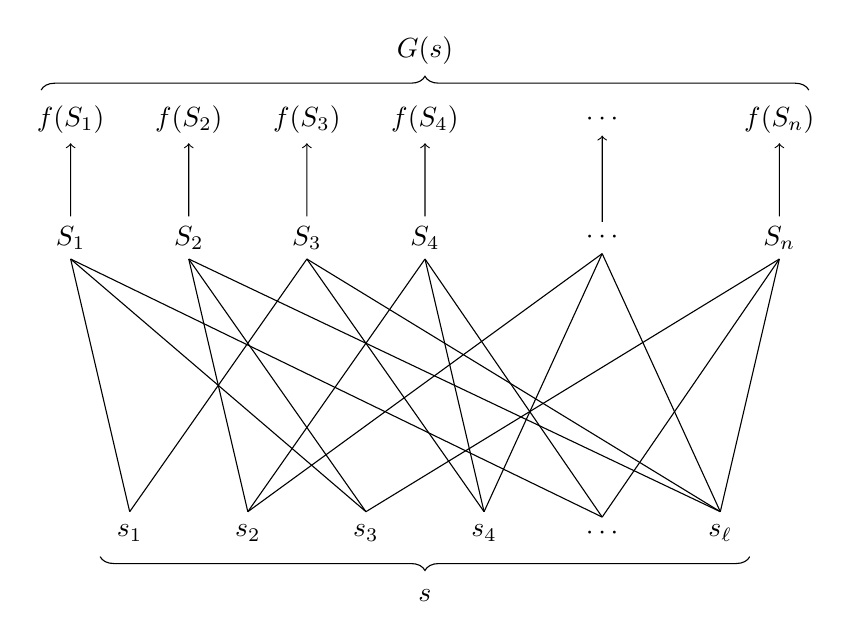
\begin{tikzpicture}[align=center,node distance=4cm, scale=1.5]
        \node[circle, inner sep=0pt, minimum size=15pt] (1) at (1, 0) {$s_1$}; 
        \node[circle, inner sep=0pt, minimum size=15pt] (2) at (2, 0) {$s_2$};
        \node[circle, inner sep=0pt, minimum size=15pt] (3) at (3, 0) {$s_3$};
        \node[circle, inner sep=0pt, minimum size=15pt] (4) at (4, 0) {$s_4$};
        \node[] (5) at (5, 0) {$\cdots$};
        \node[circle, inner sep=0pt, minimum size=15pt] (6) at (6, 0) {$s_{\ell}$};

        \node[] (11) at (.5, 2.5) {$S_1$};
        \draw[] (1.north) -- (11.south);
        \draw[] (3.north) -- (11.south);
        \draw[] (5.north) -- (11.south);

        \node[] (21) at (.5, 3.5) {$f(S_1)$};

        \draw[->] (11) -- (21);


        \node[] (12) at (1.5, 2.5) {$S_2$};
        \draw[] (2.north) -- (12.south);
        \draw[] (3.north) -- (12.south);
        \draw[] (6.north) -- (12.south);

        \node[] (22) at (1.5, 3.5) {$f(S_2)$};

        \draw[->] (12) -- (22);


        \node[] (13) at (2.5, 2.5) {$S_3$};
        \draw[] (1.north) -- (13.south);
        \draw[] (4.north) -- (13.south);
        \draw[] (6.north) -- (13.south);

        \node[] (23) at (2.5, 3.5) {$f(S_3)$};

        \draw[->] (13) -- (23);


        \node[] (14) at (3.5, 2.5) {$S_4$};
        \draw[] (2.north) -- (14.south);
        \draw[] (4.north) -- (14.south);
        \draw[] (5.north) -- (14.south);

        \node[] (24) at (3.5, 3.5) {$f(S_4)$};

        \draw[->] (14) -- (24);


        \node[] (15) at (5, 2.5) {$\cdots$};
        \draw[] (4.north) -- (15.south);
        \draw[] (2.north) -- (15.south);
        \draw[] (6.north) -- (15.south);

        \node[] (25) at (5, 3.5) {$\cdots$};

        \draw[->] (15) -- (25);

        \node[] (16) at (6.5, 2.5) {$S_n$};
        \draw[] (3.north) -- (16.south);
        \draw[] (5.north) -- (16.south);
        \draw[] (6.north) -- (16.south);

        \node[] (26) at (6.5, 3.5) {$f(S_n)$};

        \draw[->] (16) -- (26);

        \draw [decorate,decoration={brace,amplitude=5pt}]
  (0.25,3.75) -- (6.75,3.75) node[midway, yshift=.5cm]{$G(s)$};

        \draw[decorate, decoration={brace,amplitude=5pt, mirror}] 
        (.75, -.2) -- (6.25, -.2) node[midway, yshift=-.5cm]{$s$};
    \end{tikzpicture}
\end{center}

\subsection{Worst Case Hardness to Mild Hardness}

\newpage

\begin{theorem}{3.x}
    Suppose that $\cC$ is a $[m^2, m]_2$ code with the following properties:
    \begin{enumerate}
        \item the encoding map $\Enc : \pmo^m \rightarrow \pmo^{m^2}$ is computable in $\poly(m)$ time,
        \item there exists a local decoding algorithm $\LDec$ which can correct up to a relative distance of $.05$ running in $\polylog(m)$ time.
    \end{enumerate}
    Then the worst case hardness assumption implies the mild hardness assumption.
\end{theorem}

\begin{proof}

    Suppose that there exists a function $f : \pmon \rightarrow \pmo$ which can be computed in time $2^{O(n)}$ but, for some $\delta > 0$, 
    \begin{equation*}
        \Corr\left(f, 2^{\delta n}\right) < 1.
    \end{equation*}
    Having $N = 2^n$, we can represent $f$ as a string of length $N$ by its truth table $\TT(f) \in \pmo^N$. Then when we encode this string using our code $\cC$, we can view the string $\Enc(\TT(f)) \in \pmo^{2N}$ as the truth table of a function $\TT(\hat{f})$, where $\hat{f} : \pmo^{2n} \rightarrow \pmo$. We claim that for some constant $\delta' > 0$,
    \begin{equation*}
        \Corr\left(\hat{f}, 2^{\delta' n}\right) \leq .9.
    \end{equation*}
    To prove this, suppose for the sake of contradiction that there existed a circuit $C$ of size $2^{\delta' n}$ with correlation $\geq .9$ with $\hat{f}$. We will use $C$ to construct a circuit perfectly computing $f$. To start, consider the truth table $\TT(C)$ of the function computed by $C$. Because $C$ achieves high correlation with $\hat{f}$, the relative distance between $\TT(C)$ and $\TT(\hat{f})$ must be small,
    \begin{equation*}
        \delta\left(\TT(C), \TT(\hat{f})\right) < .05.
    \end{equation*}
    Thus, if we give our local decoder $\LDec$ for $\cC$ query access to $\TT(C)$, it will with probability $\sfrac{2}{3}$ output any particular bit of $\TT(f)$ in $\polylog(N) = \poly(n)$ time. Consider the following randomized circuit $C_{\sfrac{2}{3}}$ which computes $f$ with probability $\sfrac{2}{3}$. On input $x \in \pmon$, run the local decoder on $x$, simulating query access to $\TT(C)$ by querying the circuit $C$ itself,
    \begin{equation*}
        C_{\sfrac{2}{3}}(x) = \LDec^{\TT(C)}(x).
    \end{equation*}
    The size of $C_{\sfrac{2}{3}}$ depends on the running time and query complexity of $\LDec$, since each query to $\TT(C)$ is simulated by an independent copy of $C$. Since both of these quantities are $\poly(n)$, we see that 
    \begin{equation*}
        |C_{\sfrac{2}{3}}|  \leq \poly(n) + \poly(n) |C| \leq 2^{(\delta' + o(1))n}.
    \end{equation*}
    Using the fact that circuits can be derandomized with only a polynomial blow up in size, we can obtain a circuit $C'$ of size $2^{(\delta' + o(1))n}$ compute $f$ exactly. Taking $\delta' = \delta / 3$, this would contradict the fact that $f$ cannot be computed exactly by circuits of size $2^{\delta n}$. Thus, it must be true that 
    \begin{equation*}
        \Corr\left(\hat{f}, 2^{\delta n / 3}\right) \leq .9.
    \end{equation*}
    The last thing we must verify is that $\hat{f}$ can still be computed in time $2^{O(n)} = \poly(N)$. Since our encoding map $\Enc$ and $f$ are both computable in $\poly(N)$ time, $\hat{f}$ will be as well.
\end{proof}

\subsubsection{Reed-Muller and Hadamard Codes}

Theorem 3.x reduces the task of hardness amplification to finding a suitable error correcting code. The most important property of this code is that it is locally decodable. As a starting point, let's take a look at a code which has good rate, distance and is locally correctable: the Reed-Muller code.

\begin{definition}{3.x}[Reed-Muller Codes]
    Suppose $\F$ is a finite field of size $q$. The Reed-Muller code $\RM_q(m, d)$ is the set of all evaluations of $d$-degree $m$-variate polynomials over $\F_q$,
    \begin{equation*}
        \RM_q(m ,d) = \left\{(f(\gamma_1), f(\gamma_2), \ldots, f(\gamma_{q^m})) : f \in \F_q[X_1, \ldots, X_m], \, \deg (f) \leq d\right\},
    \end{equation*}
    where $\gamma_1, \ldots, \gamma_{q^m}$ is a canonical ordering of $\F_q^m$. This code has dimension $k = \binom{m + d}{d}$, block length $q^m$, and relative distance $\delta = 1 - d/ q$.
\end{definition}

In class, we saw the following guarantees for locally correcting the Reed-Muller code.

\begin{claim}{3.x}
    There exists a local corrector $\LCor_\RM$ for the Reed-Muller code $\RM_q(m, r)$ which locally corrects up to a relative distance of $\delta \leq \sfrac{1}{7}$ with $q$ queries in time $\poly(m, q, r)$.
\end{claim}

For a second, let's put aside the fact that we can only locally correct, rather than decode, this code, and let's also ignore the fact that it is a binary code. How should we pick $d$, $q$ and $m$ to achieve the regime required by Theorem 3.x? As a start, we need the number of queries to be poly-logarithmic in $n$, say $q = \log^3 n$. We'll also want the block length to be $\poly(n)$. Thus, we should take $m = \log n / \log \log n$, so that the block length is 
\begin{equation*}
    q^n = \left(\log^3 n\right)^{\log n / \log \log n} = 2^{3\log \log n \log n / \log \log n} = 2^{3\log n} = n^3.
\end{equation*}
Next, we need the dimension $k$ to be at least $n$, so that we can encode an entire string of length $n$. See that 
\begin{equation*}
    k = \binom{m + d}{d} = \binom{m + d}{m} \geq \left(\frac{m + d}{m}\right)^{m} \geq \left(\frac{d}{m}\right)^{m}.
\end{equation*}
In this case, we need to take $d = \log^2 n$, so that 
\begin{equation*}
    k \geq \left(\frac{\log^2 n \log \log n}{\log n}\right)^{\log n / \log \log n} \geq \left(\log n\right)^{\log n / \log \log n} \geq n.
\end{equation*}
Finally, the distance is $\delta = 1 - d / q = 1 - 1 / \log n$; however, since we can only locally decode up to a distance of $\delta \leq \sfrac{1}{7}$, we will take that as our distance instead. Let's call this code, with the parameters above, $\RM$. To summarize, we have that $\RM$ is a $[n^3, n, \sfrac{1}{7}]_\F$ code, where $\F$ is a finite field of size $\log^3 n$. To convert this to a binary code, we can concatenate with another code which is locally correctible: the Hadamard code.

\begin{definition}{3.x}[Hadamard Codes]
    The Hadamard code $\Had_k \subseteq \pmo^{2^k}$ with parameter $k$ is the subset of truth tables of linear functions from $\pmo^k$ to $\pmo$:
    \begin{equation*}
        \Had_k = \left\{\TT\left(x \mapsto \prod_{i \in S} x_i\right) : S \subseteq [k]\right\}.
    \end{equation*} 
    This code has dimension $k$, block length $2^k$, and relative distance $\delta = \sfrac{1}{2}$.
\end{definition}

In class, we saw the following guarantees for locally correcting the Hadamard code.

\begin{claim}{3.x}
    There exists a local corrector $\LCor_\Had$ for the Hadamard code $\Had_k$ which locally corrects up to a relative distance of $\delta \leq \sfrac{1}{4}$ with $2$ queries in time $O(k)$.
\end{claim}

Fixing $k = \log |\F|$, we will write $\Had$ for the Hadamard code with parameter $k$. Let's suppose for a second that we could transform each of our local correcting algorithms to local decoding algorithms. Then we claim that the concatenated code $\cC = \Had \concat \RM$ will satisfy the requirements of Theorem 3.x.

\begin{claim}{3.x}
    The code $\cC$ is a $[n^3\log^3 n, n]_2$ code which can be locally decoded up to a relative distance of $\sfrac{1}{28}$ in $\polylog(n)$ time.
\end{claim}

\begin{proof}
    Let's begin by verifying the parameters of the code. The dimension will still by $n$. To compute the block length, see that every symbol of a codeword $c \in \RM$ is encoded to a Hadamard codeword of length $2^{\log |\F|} = |\F| = \log^3 n$, so that the total length of the resulting word is $n^3 \log^3 n$. Thus, $\cC$ is indeed a $[n^3 \log^3 n, n]_2$ code.

    Next, we claim that $\cC$ can be locally decoded in time $\polylog(n)$ up to a distance of $\sfrac{1}{28}$. Suppose that $c \in \cC$ and $\tilde{c}$ is a corrupted codeword such that $\delta(c, \tilde{c}) \leq \sfrac{1}{28}$. The algorithm for locally recovering $c$ from $\tilde{c}$ runs as follows. Run the local decoder $\LDec_\RM$ on the Reed-Muller code word represented by $\tilde{c}$, replacing each query to this code word with a call to the local decoder $\LDec_\Had$ with query access to $\tilde{c}$.

    To see why this is a good idea, consider that since $\delta(c, \tilde{c}) \leq \sfrac{1}{28}$, there can be at most a $\sfrac{1}{7}$ blocks of Hadamard codewords which are corrupted beyond a distance of $\sfrac{1}{4}$. Thus the local decoder $\LDec_\Had$ with be able to decode a $1 - \sfrac{1}{7}$ fraction of these blocks. Therefore, the codeword which $\LDec_\RM$ queries will have distance at most $\sfrac{1}{7}$ from the polynomial represented by $c$, and thus it will locally decode $c$ with high probability.
    
    Note that this will still run in time poly-logarithmic in $n$. Furthermore, we can boost the success probability of each decoder by repetition by sacrificing only a small increase in run time, and thus the process above can be made to succeed with probability $\sfrac{2}{3}$. Thus, $\cC$ can be locally decoded in $\polylog(n)$ time.
\end{proof}

So, given two local decoding algorithms for $\Had$ and $\RM$, we can construct our desired code. To convert our local correctors to local decoders, recall the notion of systematic encodings.

\begin{definition}{3.x}
    A $[\ell, n]_2$  code with encoder $\Enc : \pmo^{n} \rightarrow \pmo^{\ell}$ is systematic if for every bit $i_{in} \in [n]$, there exists a bit $i_{out} \in [\ell]$ such that for any message $w \in \pmon$, 
    \begin{equation*}
        (\Enc(w))_{i_{out}} = w_{i_{in}}.
    \end{equation*}
\end{definition}

In other words, a systematic encoding of a code allows one to obtain any bit in the original message by reading a particular bit of the codeword. Thus, if a code is both locally correctable and systematically encodable, then we can systematically decode it, since to recover a particular index of the message, we just need to locally correct the corresponding index in the corrupted code word. Thus, we just need to find systematic encodings for both $\Had$ and $\RM$.

\subsubsection{Systematic Encodings and Low Degree Extensions}

First, we claim that the standard encoder for the Hadamard code is systematic. Recall that given a string $w \in \zo^k$, the encoder $\Enc_\Had : \zo^k \rightarrow \zo^{2^k}$ just outputs the truth table of the function $x \mapsto \langle x, w \rangle$,
\begin{equation*}
    \Enc_\Had (w) = \TT\left(x \mapsto \langle x, w \rangle\right).
\end{equation*}
In particular, in the index corresponding to $x = e_i$, the value of $\Enc_\Had(w)$ is just $\langle w, e_i \rangle = w_i$. Thus, this encoding is systematic, and we obtain a local decoder for $\Had$.

\begin{claim}{3.x}
    The Hadamard code $\Had$ can be efficiently, systematically encoded, and locally decoded up to a relative distance of $\delta \leq \sfrac{1}{4}$ with $2$ queries.
\end{claim}

However, we have to be a bit more careful with the Reed-Muller code. The encoder we saw in class views the message as coefficients of a low degree polynomial, while the encoded word is the value of that polynomial on every input. To systematically encode the Reed-Muller code, we will need to view the message as a subset of these evaluation points, and transform these into a polynomial which takes the same values on these points. Before specifying exactly what we mean by this, let's recall our setup from the section above: our code $\RM$ was a Reed-Muller code $\RM_q(m, d)$, where $q = \log^3 n$, $m = \log n / \log \log n$, and $d = \log^2 n$. This code had dimension at least $n$, so that we can encode any $w \in \zo^n$ to a codeword $c \in \RM_q(m, d)$. To following claim gives a way to systematically encode $\RM$.

\begin{claim}{3.x}
    Our Reed-Muller code $\RM$ can be efficiently systematically encoded.
\end{claim}

\begin{proof}
    Fix a subset $\bH \subseteq \F_q$ of size $|\bH| = \log n$. The proof works as follows: first, we show that any $w \in \zo^n$ can be viewed as the truth table of a function $f_w : \bH^m \rightarrow \zo$. Next, we show that any such $f : \bH^m \rightarrow \zo$ can be extended to a codeword $\hat{f}_w : \F_q^m \rightarrow \F_q$ in $\RM$ which agrees with $f$ on the subset $\bH^m$. Once we prove both of these steps, the encoding which maps $w \in \zo^n$ to the evaluation of $\hat{f}_w$ will be systematic. Fix some $w \in \zo^n$. See that the set $\bH^m$ has size 
    \begin{equation*}
        |\bH^m| = \left(\log n\right)^{\log n / \log \log n} = n.
    \end{equation*}
    Thus, any $w \in \zo^n$ represents the truth table of a $f_w : \bH^m \rightarrow \zo$, and vice versa. Next, suppose we have some $f_w : \bH^m \rightarrow \zo$. Consider the polynomial $\hat{f}_w : \F_q^m \rightarrow \F_q$ defined by 
    \begin{equation*}
        \hat{f}_w(X_1, \ldots, X_m) = \sum_{\alpha \in \bH^m} f_w(\alpha) \cdot \frac{\delta_\alpha \left(X_1, \ldots, X_m\right)}{\delta_\alpha(\alpha)},
    \end{equation*}
    where we define 
    \begin{equation*}
        \delta_\alpha \left(X_1, \ldots, X_m\right) = \prod_{i \in [m]} \prod_{\gamma \in \bH \setminus \{\alpha_i\}} (X_i - \gamma). \tag{1}
    \end{equation*}
    We claim that $\hat{f}_w |_{\bH^m} = f_w$. First, note that for any $\alpha, \beta \in \bH^m$, $\delta_{\alpha}(\beta) = 0$ unless $\alpha = \beta$. To see why, consider that if $\alpha \neq \beta$, then there exists a particular index $j \in [m]$ where $\alpha$ and $\beta$ differ, so that $\beta_j \notin \bH \setminus \{\alpha_j\}$. Then the product in equation (1) contains a $(\beta_j - \beta_j)$ term, and thus is equal to $0$. With this observation, we see that for any $\beta \in \bH^m$, 
    \begin{equation*}
        \hat{f}_w \left(\beta\right) = \sum_{\alpha \in \bH^m} f_w(\alpha) \frac{\delta_\alpha(\beta)}{\delta_{\alpha}(\alpha)} = f_w(\beta) \frac{\delta_\beta(\beta)}{\delta_\beta(\beta)} = f_w(\beta).
    \end{equation*}
    Thus, $\hat{f}_w$ does extend $f_w$ on $\bH^m$. To complete the proof, we have to verify that $\hat{f}_w$ is a codeword in $\RM$. To do so, we just need to verify that $\deg(\hat{f}_w) \leq d = \log^2 n$. By construction, the degree of $\hat{f}_w$ is at most the degree of any $\delta_\alpha(X_1, \ldots, X_m)$. Since each $\delta_\alpha$ is the product of $m \cdot (|\bH| - 1)$ monomials, the degree of $\hat{f}_w$ is,
    \begin{equation*}
        \deg \left(\hat{f}_w\right) \leq m \cdot (|\bH| - 1) \leq \frac{\log n}{\log \log n} \cdot \left(\log n - 1\right) \leq \log^2 n = d.
    \end{equation*}
    Thus, our encoding will map $w \in \zo^n$ to codewords $\hat{f}_w \in \RM$ systematically. Note also that this encoding is still efficient, since the polynomial $\hat{f}_w$ can be evaluated in at any $\beta \in \F_q^m$ in $\poly(m, q, d)$ time.
\end{proof}

\subsection{Worst Case Hardness to Average Case Hardness}

Note that in our analysis in Theorem 3.?, we could amplify the hardness of the any function $f$ to $1 - \delta$, where $\delta$ is the relative distance of the code $\cC$ at which we can locally decode it. However, since $\cC$ must be binary, $\delta \leq \sfrac{1}{2}$, and so local decoding can not get us to exponentially small correlation. To break past this barrier, we can use list decoding. 

\begin{theorem}{3.x}
    The average case hardness assumption implies the worst case hardness assumption.
\end{theorem}



\section{Boosting and Hardness Amplification}

\subsection{Smooth Boosters and The Hardcore Theorem}

\begin{center}
    \begin{tikzpicture}
        \path[draw] (-6.5, -2) rectangle (-2.5, 2);
        \path[draw,use Hobby shortcut,closed=true, pattern=north east lines]
        (-4,.3) .. (-4.4,.4) .. (-5.6, -.3);
        \node[fill=white] at (-4.6, -.5) {$H_1$};
        \node[] at (-4.5, 2.35) {$C_1$};


        \path[draw] (-2, -2) rectangle (2, 2);
        \path[draw,use Hobby shortcut,closed=true, pattern=north east lines]
        (0,.3) .. (.4,1) .. (.6,1.6) .. (1.4,1.4) .. (1.6, .3);
        \node[fill=white] at (.9, .7) {$H_2$};
        \node[] at (0, 2.35) {$C_2$};

        \path[draw] (2.5, -2) rectangle (6.5, 2);
        \path[draw,use Hobby shortcut,closed=true, pattern=north east lines]
        (4,.3) .. (4.4,.5) .. (5.6, -.3);
        \node[fill=white] at (4.7, -.3) {$H_3$};
        \node[] at (4.5, 2.35) {$C_3$};

        \draw[decorate, decoration={brace,amplitude=5pt, mirror}] 
        (-6.75, -2.25) -- (6.75, -2.25) node[midway, yshift=-.5cm]{};

        \draw[->] (0, -2.4) -- (0, -2.8);

        \path[draw] (-2, -7) rectangle (2, -3);
        \path[draw,use Hobby shortcut,closed=true, pattern=north east lines]
        (-.1,-5) .. (.4,-4.4) .. (1.6, -4.7);
        \node[fill=white] at (.8, -5) {$H$};
    \end{tikzpicture}
\end{center}

\subsection{Boosting via the XOR Lemma}



\end{document}